% \documentclass[dvipdfmx, 11pt]{beamer}
\documentclass[aspectratio=169, dvipdfmx, 11pt]{beamer} % aspectratio=43, 149, 169
\usepackage{here, amsmath, latexsym, amssymb, bm, ascmac, mathtools, multicol, tcolorbox, subfig, bookmark}

% デザイン
\usetheme{Luebeck}
\usecolortheme{orchid}
\usefonttheme{professionalfonts}
\useinnertheme{circles}
\useoutertheme{infolines}
\setbeamercolor{title}{fg=structure, bg=}
\setbeamercolor{frametitle}{fg=structure, bg=}
\setbeamertemplate{itemize item}{\small\raise0.5pt\hbox{$\bullet$}}
\setbeamertemplate{itemize subitem}{\tiny\raise1.5pt\hbox{$\blacktriangleright$}}
\setbeamertemplate{itemize subsubitem}{\tiny\raise1.5pt\hbox{$\bigstar$}}

%しおりの文字化け解消
\usepackage{atbegshi}
\ifnum 42146=\euc"A4A2
\AtBeginShipoutFirst{\special{pdf:tounicode EUC-UCS2}}
\else
\AtBeginShipoutFirst{\special{pdf:tounicode 90ms-RKSJ-UCS2}}
\fi

\setbeamertemplate{navigation symbols}{}
\renewcommand{\kanjifamilydefault}{\gtdefault}
\newcommand{\red}[1]{\textcolor{red}{#1}}
\newcommand{\green}[1]{\textcolor{green!40!black}{#1}}
\newcommand{\blue}[1]{\textcolor{blue!80!black}{#1}}

\title[Day02]{機械学習の基礎}
\subtitle{Day02}
\author[Yudai Fujimoto]{Yudai Fujimoto}
\institute[SUS]{Suwa University of Science}
\date{\today}

\begin{document}
\maketitle

\begin{frame}{目次}
    \tableofcontents
\end{frame}

\section{パーセプトロンの欠点}
\begin{frame}{パーセプトロンの欠点}
    パーセプトロンによって分類ができることは判明したが、視覚的には何を行っているか。 \\
    分類結果を図に表すと特徴量を下の式を満たす超平面で区切っていることがわかる。 \\
    \begin{equation*}
        \bm{W} \bm{x} = 0
    \end{equation*}
    \begin{figure}[b]
        \begin{center}
        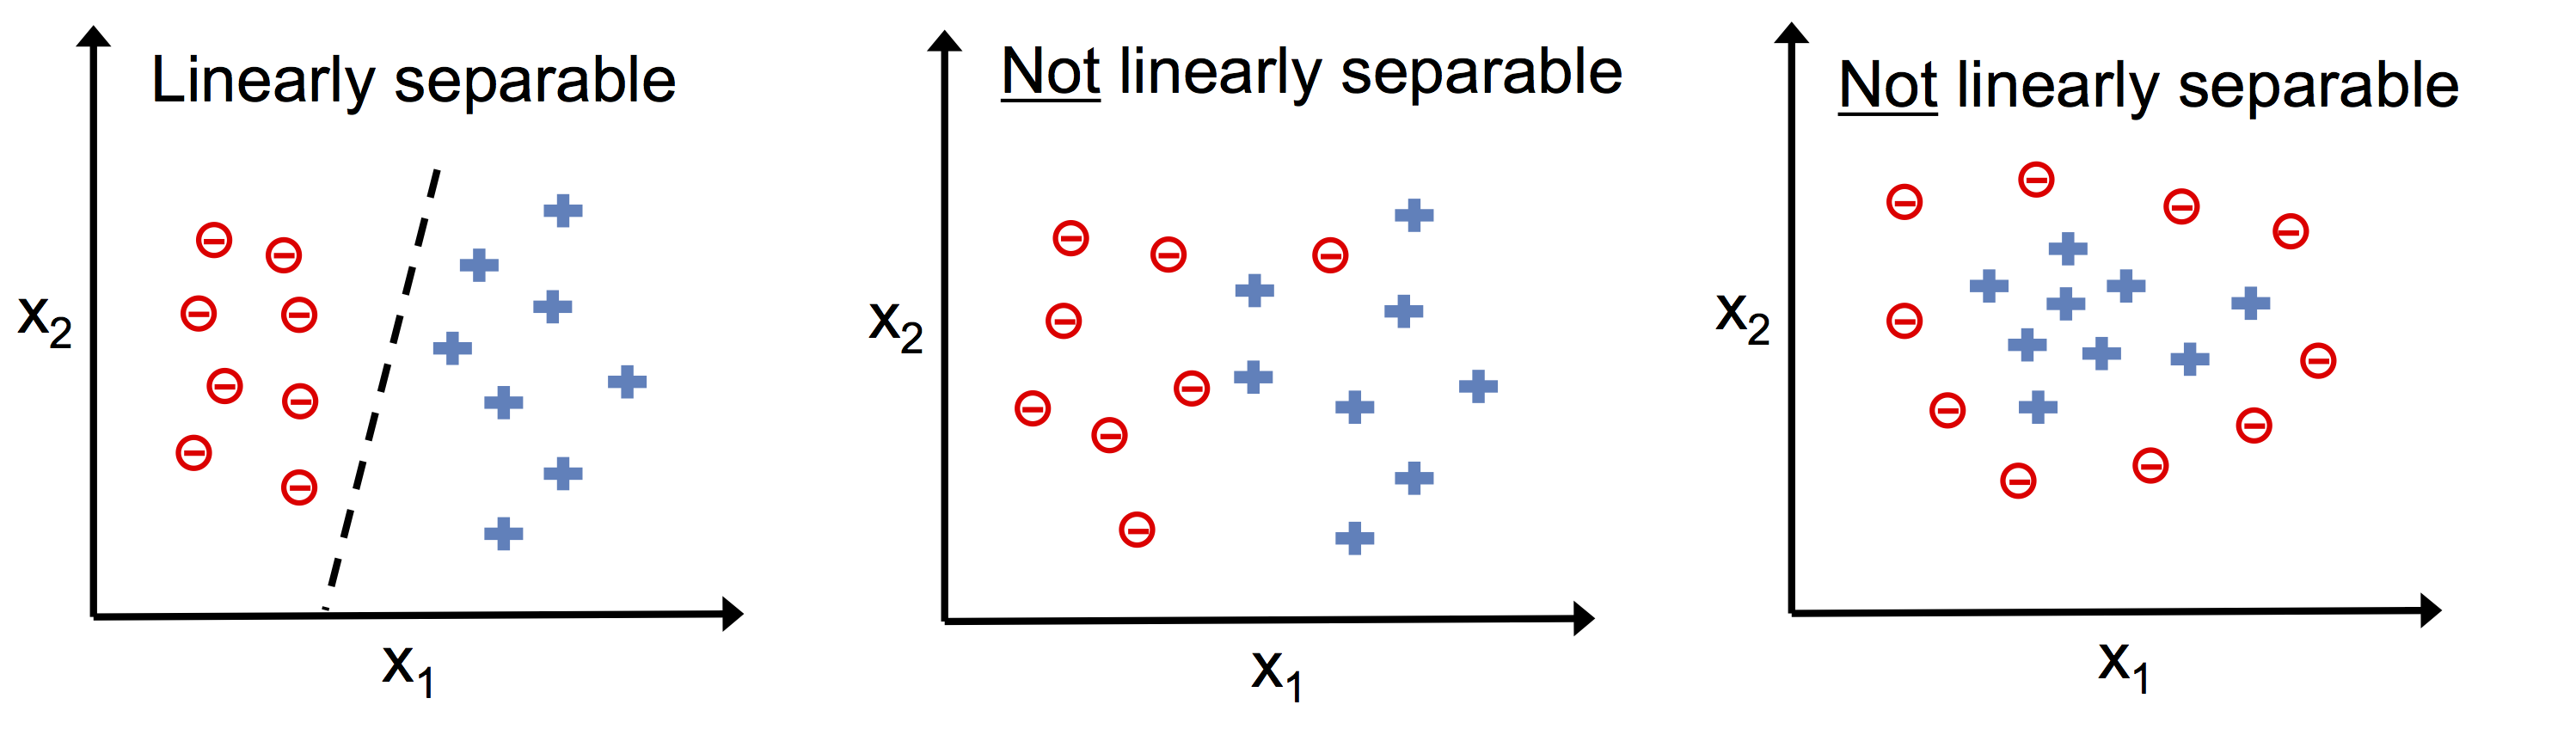
\includegraphics[width=120mm]{img/day02/fig01.png}
        \end{center}
    \end{figure}
    しかし、すべてのデータを完璧に分類できるとは限らないので別のアルゴリズムを試す。
\end{frame}

\section{ロジスティック回帰}
\begin{frame}{ロジスティック回帰}
    パーセプトロンではクラスが1か-1かのみで分類していたが、
    これでは線形分離できなかった場合に学習が収束しなくなる。
    そこで、クラスに属する確率を予測するロジスティック回帰(Logistic regression)
    を見ていく。
    ロジスティック回帰モデルは名前とは裏腹に分類のためのモデルである。
\end{frame} 

\begin{frame}{logit関数}
    ロジスティック回帰の核となるオッズ比を紹介する。\\
    オッズ比は予測したい事象の起こりやすさを表し、下の式で表される。
    \begin{equation*}
        Odds Raito = \frac{p}{(1-p)}
    \end{equation*}
    正事象については、クラスラベル\(y=1\)として考えることができる。
    その場合はロジット(logit)関数を定義できる。この関数は単にオッズ比の対数。
    \begin{equation*}
        logit(p) = log(OddsRaito) = log(\frac{p}{1-p})
    \end{equation*}
    ロジット関数はp\((0\leq p \leq 1)\)を受け取って実数全体の範囲に変換する。
    \rightline{\footnotesize ※\(log\)は自然対数。}
\end{frame} 

\begin{frame}{sigmoid関数}
    ロジット関数を使うことで特徴量と対数オッズの線形関係を表すことができる。
    \begin{equation*}
        logit(p(y=1 \mid \bm{x})) = x_0w_0 + x_1w_1 + \cdots  + x_mw_m = \bm{w^T}\bm{x}
    \end{equation*}
    ここで\(p(y=1 \mid \bm{x})\)は特徴量\(x\)が与えられた場合にデータがクラス1に属する条件付き確率。
    実際に関心があるのが、データが特定のクラスに所属している確率を予測することである。
    これはロジット関数の逆関数であるロジスティックシグモイド関数で実現できる。
    \begin{equation*}
        \phi(z) = \frac{1}{1+e^{-z}}
    \end{equation*}
    ここで\(z\)は総入力である。つまり重み\(\bm{w}\)と入力\(\bm{x}\)の線形結合で以下のように表される。
    \begin{equation*}
        z = \bm{w^T}\bm{x} = x_0w_0 + x_1w_1 + \cdots  + x_mw_m
    \end{equation*}
\end{frame}

\begin{frame}{sigmoid関数}
    \(-7 \leq z \leq  7\)の範囲のsigmoid関数をプロットするとS字型曲線が表示される。 \\
    それにより、sigmoid関数は入力として実数値を受け取り、\(\phi(z)=0.5\)を切片として、
    その入力値を\([0, 1]\)の範囲に変換することを結論づけることができる。
    \begin{figure}[b]
        \begin{center}
        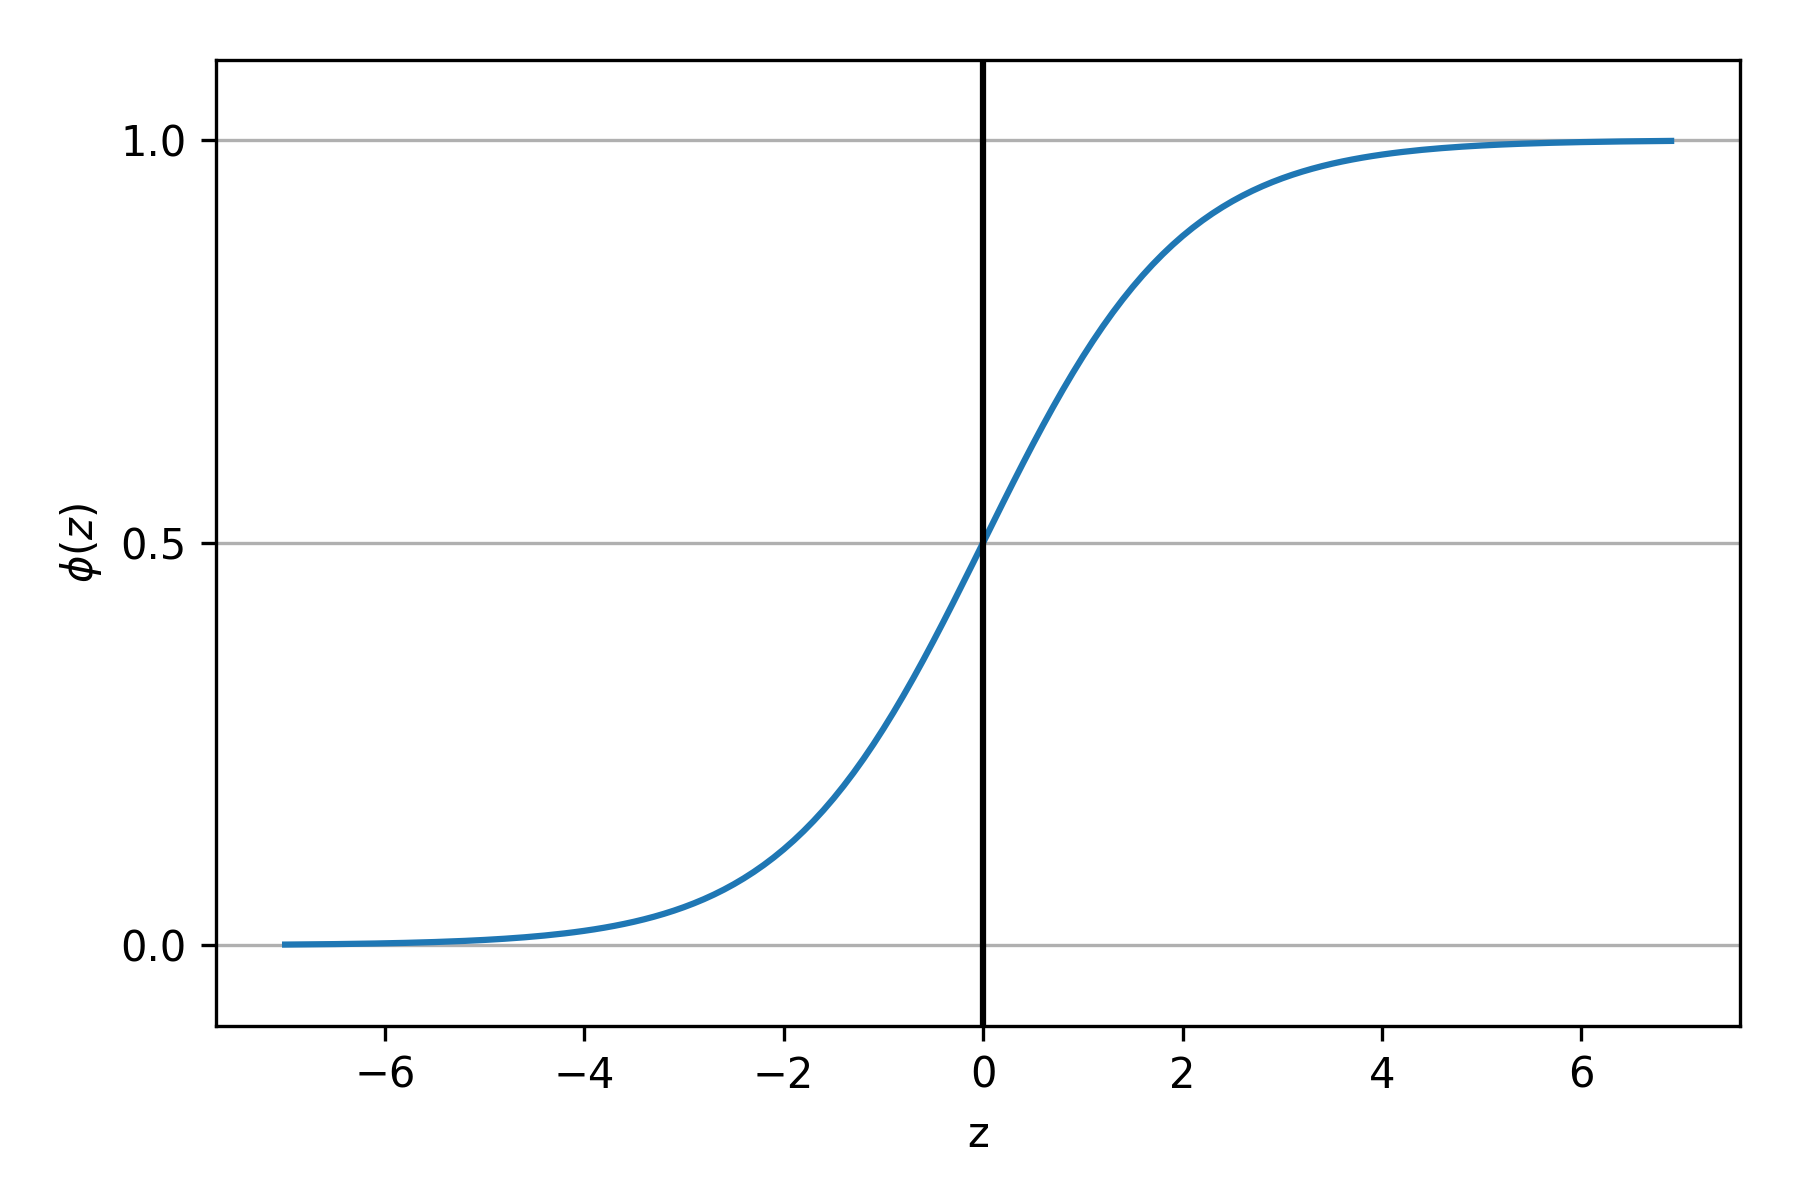
\includegraphics[width=80mm]{img/day02/fig02.png}
        \end{center}
    \end{figure}
\end{frame}

\begin{frame}{ロジスティック回帰}
    ロジスティック回帰モデルの構造を下図に示す。 \\
    このシグモイド関数の出力はデータがクラス1に属している確率\(P(y=1 \mid x;w)\)である。 \\
    例えばあるデータに対して\(\phi(z)=0.8\)が算出された場合はIris-Versicolorである確率が80\%であることを意味する。
    あとは閾値関数を用いて二値の成果仕様に変換すれば良い。
    \begin{figure}[b]
        \begin{center}
        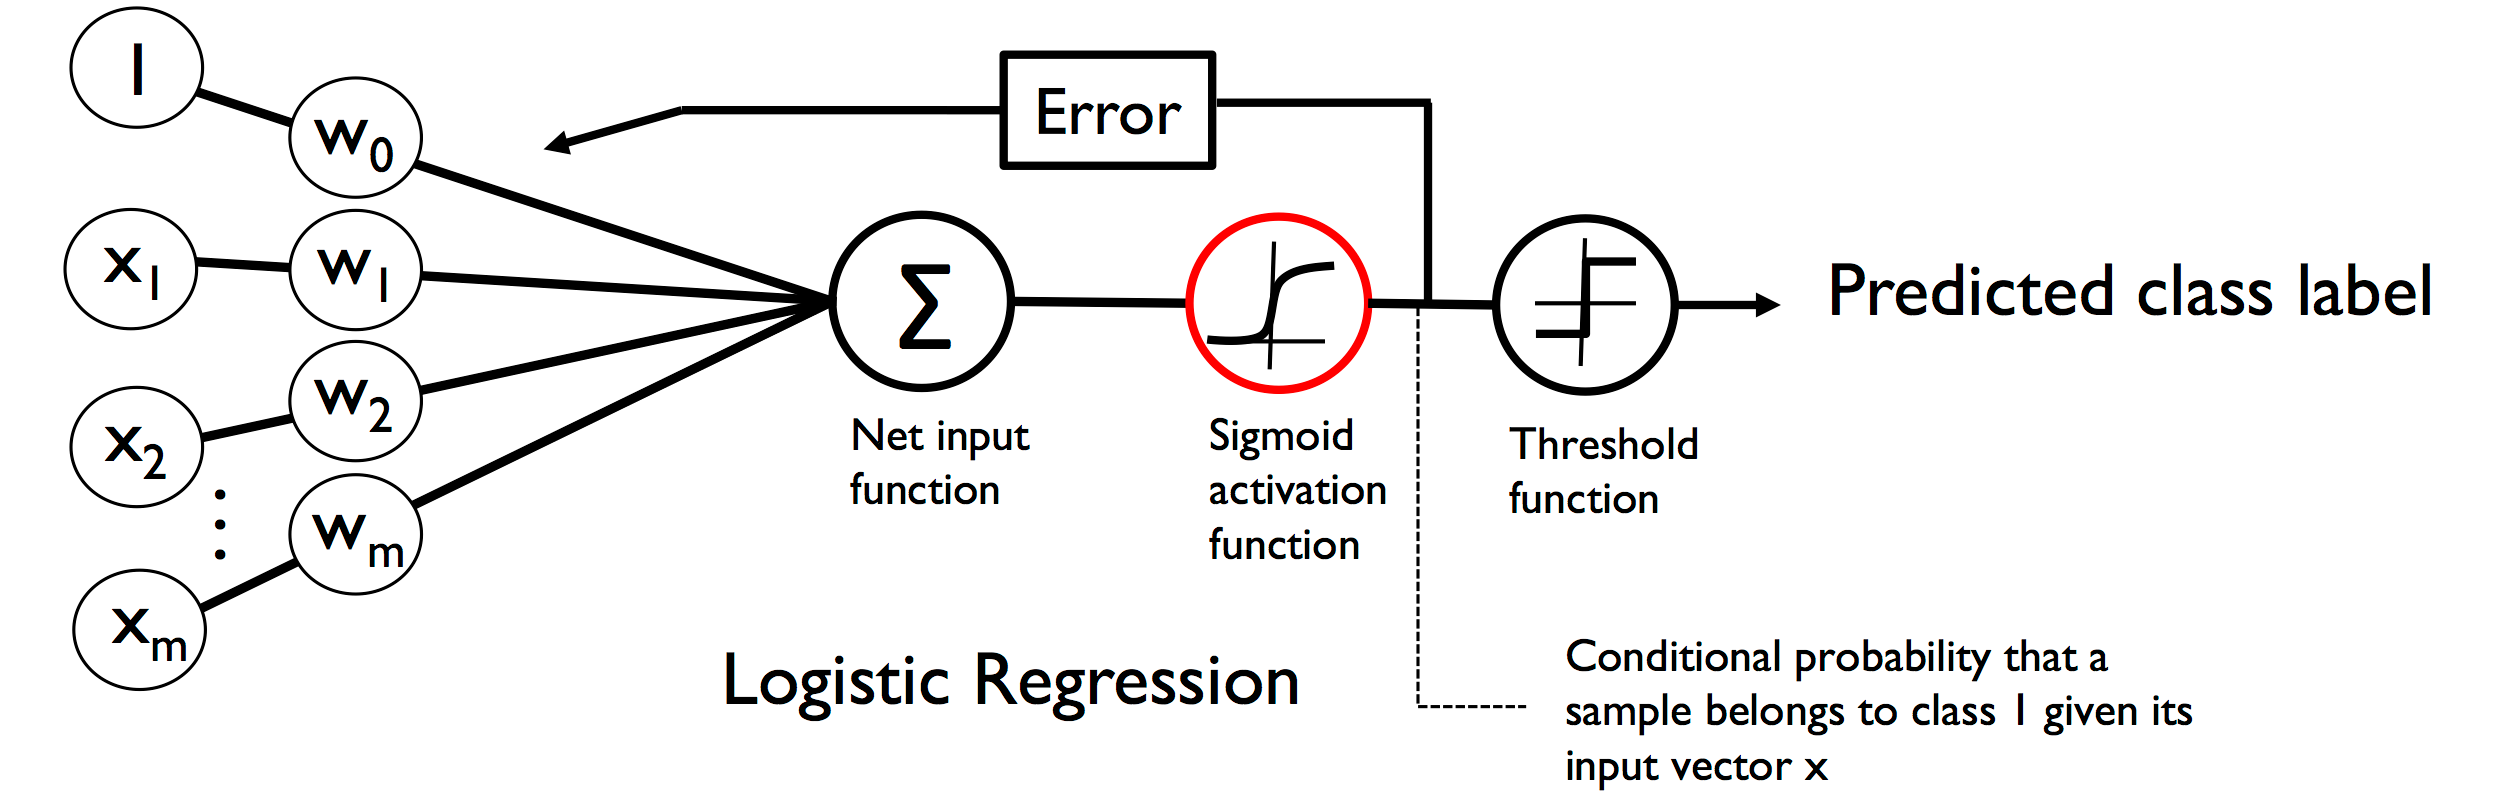
\includegraphics[width=100mm]{img/day02/fig03.png}
        \end{center}
    \end{figure}
    \begin{equation*}
        \hat{y} = 
        \begin{aligned}
            & \left\{ \,
                \begin{aligned}
                    & 1 & \quad &(\phi(z) \geq 0.5) \\
                    & 0 & \quad &(\phi(z) < 0.5)
                \end{aligned}
            \right.
        \end{aligned}
    \end{equation*}
\end{frame}

\begin{frame}{重みの学習}
    ロジスティック関数の損失関数の導出を説明するために、データセット中のデータが互いに
    独立だと仮定して、ロジスティック回帰モデルの構築の際に最大化したい尤度\(L\)(ゆうど: 結果から見た条件のもっともらしさ)
    を定義する。
    \begin{equation*}
        L(\bm{w}) = P(y \mid \bm{x};\bm{w})
        = \prod_{i=1}^n P(y^{(i)} \mid x^{(i)};\bm{w})
        = \prod_{i=1}^n (\phi (z^{(i)}))^{y^{(i)}} (1-\phi (z^{(i)}))^{1-y^{(i)}}
    \end{equation*}
    尤度は非常に小さくなる可能性があるので対数関数を適用する。\\
    次に係数の積を係数の和に変換すると加算を用いて導関数を簡単に得ることができる。
    \begin{equation*}
        l(\bm{w}) = logL(\bm{w})
        = \sum_{i=1}^{n} [y^{(i)} log(\phi (z^{(i)})) + (1-y^{(i)})log(1-\phi (z^{(i)}))]
    \end{equation*}
    これで勾配上昇法などのアルゴリズムを用いて対数尤度を最大化できるようになった。
\end{frame}

\begin{frame}{重みの学習}
    勾配上昇方のかわりの方法として勾配降下法を利用するために、最小化できる損失関数\(J\)
    として対数尤度を書き直すと次のようになる。
    \begin{equation*}
        J(\bm{w}) = -logL(\bm{w})
        = \sum_{i=1}^{n} [-y^{(i)} log(\phi (z^{(i)})) - (1-y^{(i)})log(1-\phi (z^{(i)}))]
    \end{equation*}
    この損失関数の理解のために、単一の学習データに対して計算されるコストを見てみる。
    \begin{equation*}
        J(\phi (z), y;\bm{w}) = -y log(\phi (z)) - (1-y)log(1-\phi (z))
    \end{equation*}
    \begin{equation*}
        J(\phi (z), y;\bm{w}) = 
        \begin{aligned}
            & \left\{ \,
                \begin{aligned}
                    & - log(\phi (z)) & \quad &(y=1) \\
                    & - (1-y)log(1-\phi (z)) & \quad &(y=0)
                \end{aligned}
            \right.
        \end{aligned}
    \end{equation*}
    \(y=0\)であれば1つ目の項が0になり,\(y=1\)であれば2つ目の項が0になる事がわかる。
\end{frame}

\begin{frame}{重みの学習}
    さまざまな\(\phi(z)\)の値に対する単一の訓練データに対する分類コストを表すグラフを示す。\\
    データが1または0に所属していることを予想した場合にはコストが0に近づいていくことがわかる。
    ただし、予測を間違えた場合は徐々に損失を引き上げることでペナルティを課す。
    \begin{figure}[b]
        \begin{center}
        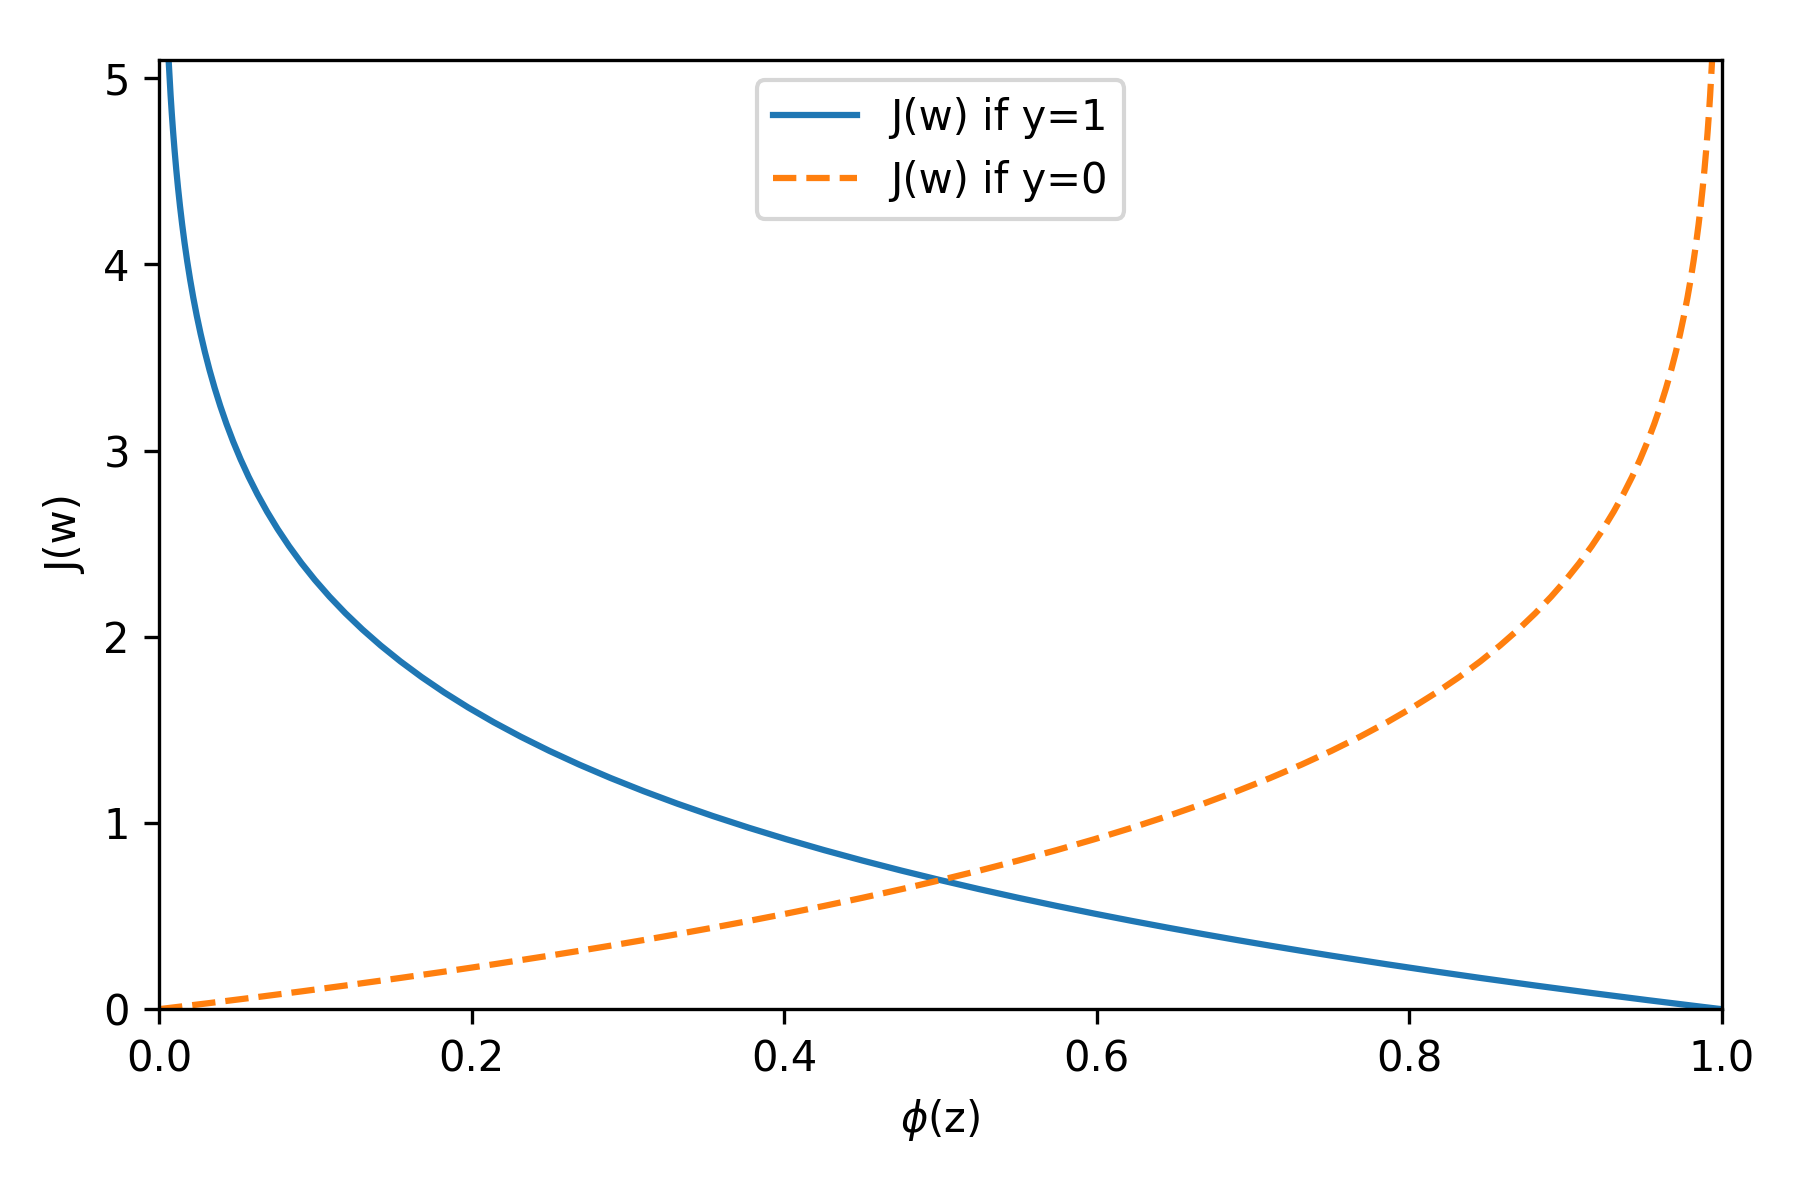
\includegraphics[width=80mm]{img/day02/fig04.png}
        \end{center}
    \end{figure}
\end{frame}

\begin{frame}{ロジスティック回帰での勾配降下法}
    導出過程は省略するが、\(j\)番目の重みに対する偏導関数は次のようになる。
    \begin{equation*}
        \frac{\partial}{\partial w_j}J(\bm{w}) = (y - \phi(z))x_j
    \end{equation*}
    % したがって、各重みの更新式は次のようになる。
    % \begin{equation*}
    %     w_j := w_j + \eta \sum_{i=1}^{n} (y^{(i)} - \phi(z^{(i)}))x_{j}^{(i)}
    % \end{equation*}
    対数尤度の最大化は、先に定義した損失関数\(J\)を最小化することに等しい。\\
    このため、勾配降下法の更新手順を次のように記述できる。
    \begin{equation*}
        \Delta w_j := - \eta \frac{\partial J}{\partial w_j} 
        = \eta \sum_{i=1}^{n} (y^{(i)} - \phi(z^{(i)}))x_{j}^{(i)}
    \end{equation*}
    \begin{equation*}
        \bm{w} := \bm{w} + \Delta \bm{w}, \Delta \bm{w} = - \eta \frac{\partial J}{\partial w_j} 
    \end{equation*}
    これはパーセプトロンの勾配降下法の規則に相当する。
\end{frame}

\section{Liner SVM}
\begin{frame}{最大マージン分類}
    サポートベクトルマシン(Support Vector Machine : SVM)は広く利用されている強力なアルゴリズムである。
    ロジスティック回帰では誤分類率を最小化したが、SVMでの目的はマージン(Margin)を最大化することである。\\
    マージンは超平面(決定境界)と、この超平面に最も近い訓練データの距離として定義される。
    このとき、超平面に最も近い訓練データをサポートベクトル(Support Vector)と呼ぶ。
    \begin{figure}[b]
        \begin{center}
        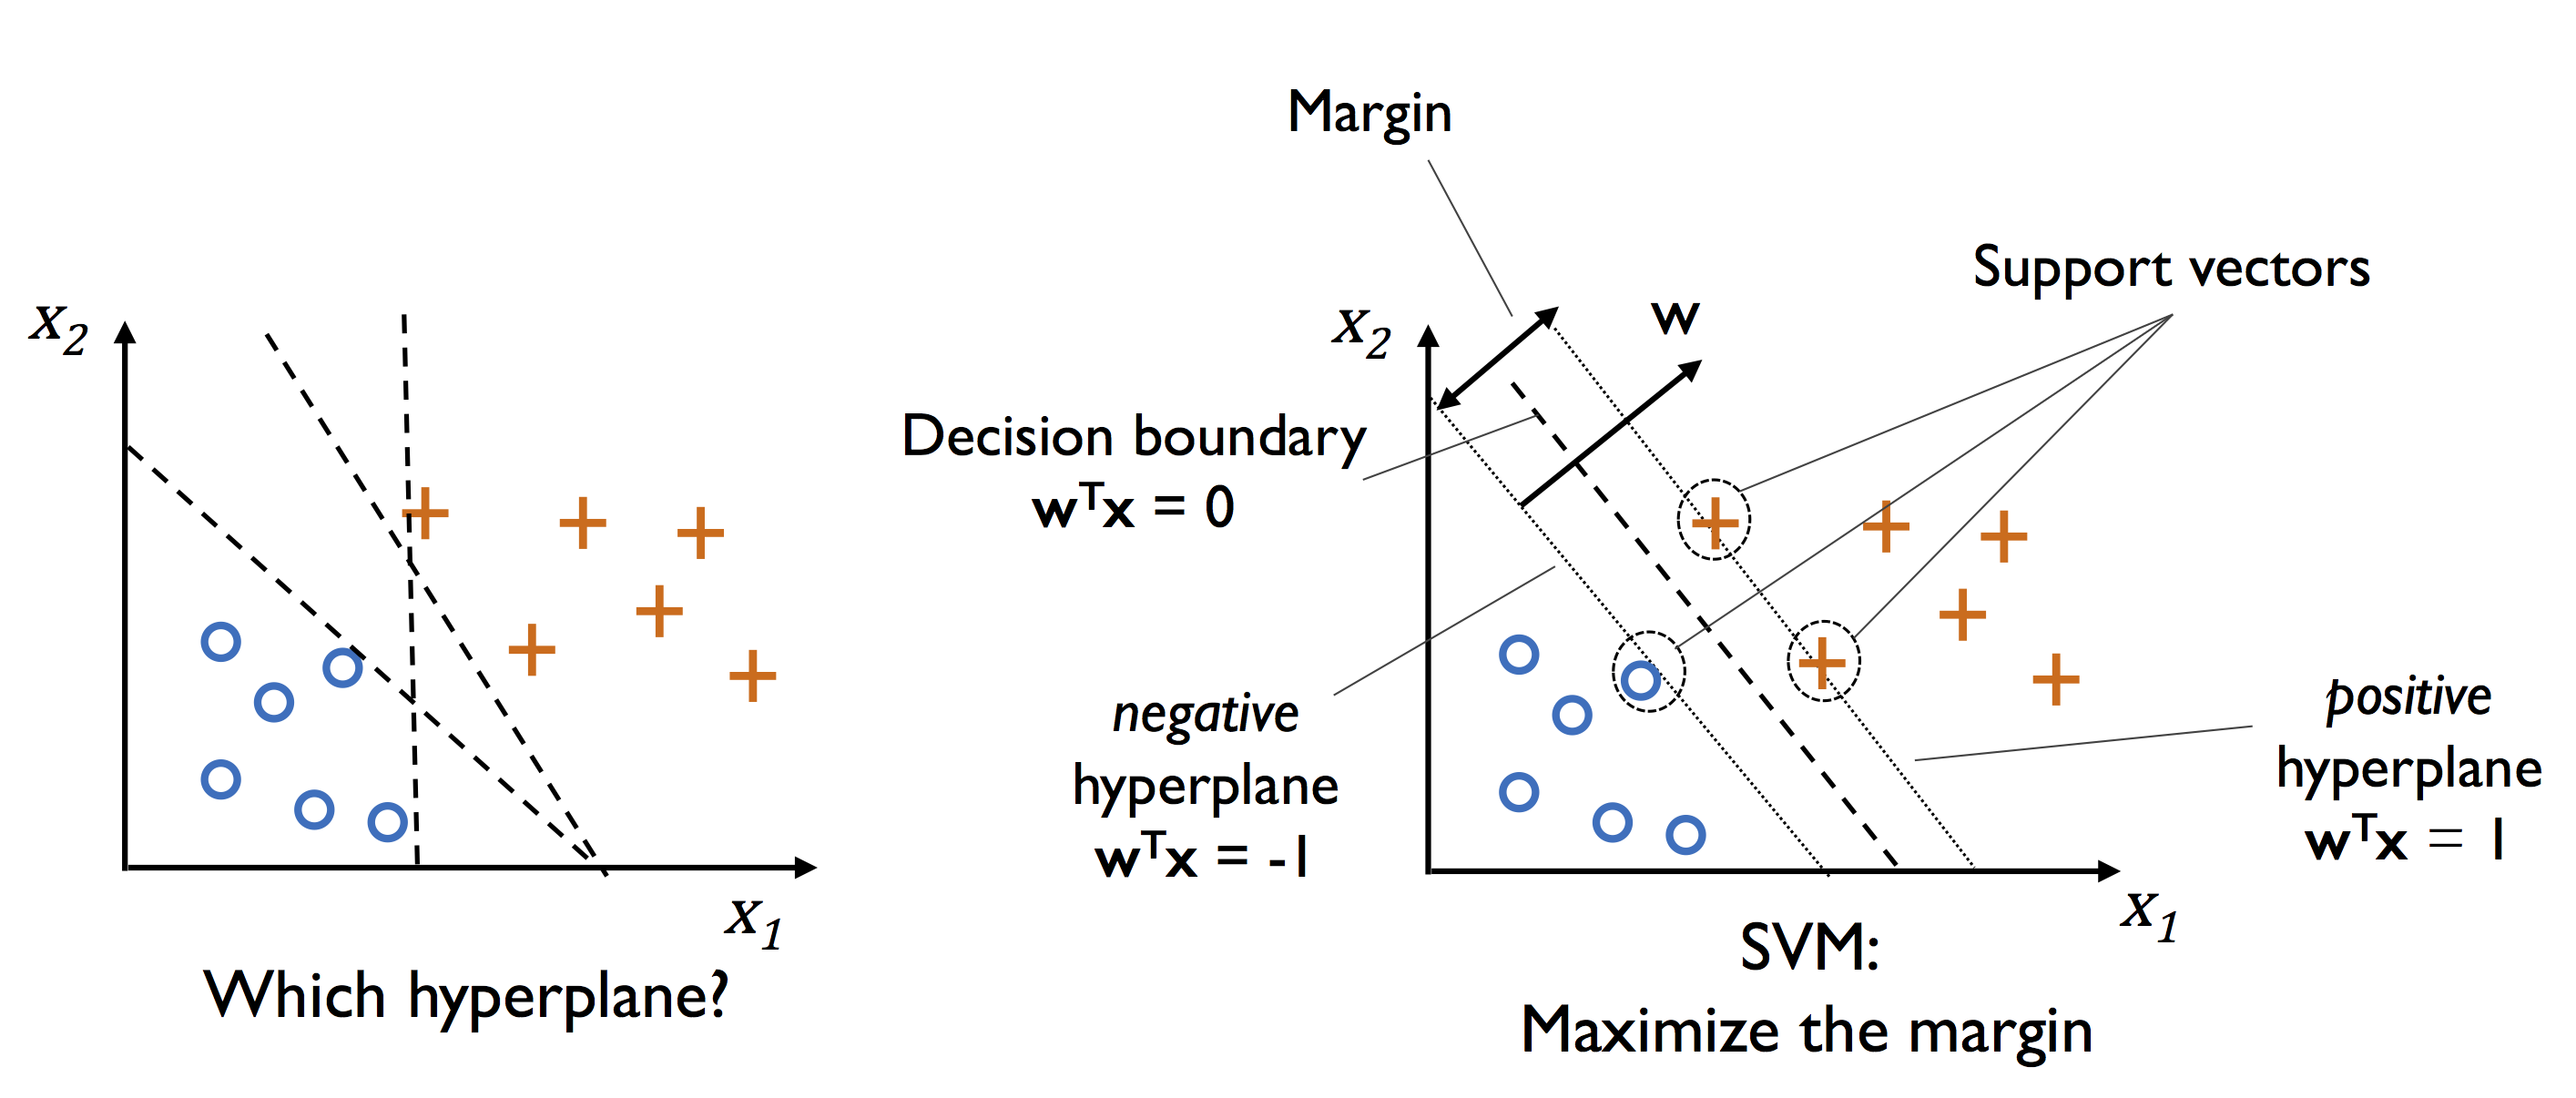
\includegraphics[width=110mm]{img/day02/fig05.png}
        \end{center}
    \end{figure}
\end{frame}

\begin{frame}{最大マージン分類}
    決定境界のマージンを大きくする利点は、汎化誤差が小さくなる傾向にあることだ。
    サポートベクトルに接した2つの超平面は次のように表すことができる。
    \begin{equation*}
        \begin{aligned}
            & \left\{ \,
                \begin{aligned}
                    & w_0 + \bm{w}^T \bm{x}_{pos} = 1 \\
                    & w_0 + \bm{w}^T \bm{x}_{neg} = -1
                \end{aligned}
            \right.
        \end{aligned}
    \end{equation*}
    これらを引き算すると次のようになる。
    \begin{equation*}
        \bm{w}^T (\bm{x}_{pos} - \bm{x}_{neg}) = 2
    \end{equation*}
    ここで、標準化を行うためにベクトルの長さを定義する。
    \begin{equation*}
        \Vert\bm{w}\Vert = \sqrt{{\textstyle \sum_{j=1}^{m} w_{j}^{2}}}
    \end{equation*}
\end{frame}

\begin{frame}{最大マージン分類}
    ここで、ベクトルの長さをもとに式を標準化すると次の式が得られる。
    \begin{equation*}
        \frac{\bm{w}^T (\bm{x}_{pos} - \bm{x}_{neg})}{\Vert\bm{w}\Vert} = \frac{2}{\Vert\bm{w}\Vert}, 
    \end{equation*}
    この式の左辺は、正負の超平面間の距離として解釈することができる。\\
    これによって、正しく分類されたデータのもとで、SVMの目的関数を最大化する問題は
    \(\frac{2}{\Vert\bm{w}\Vert}\)、すなわちマージンを最大化する問題に帰着できる。\\
    しかし、実際には\(\frac{2}{\Vert\bm{w}\Vert}\)を最大化するのでなく、
    逆数をとって二乗した\(\frac{1}{2}\Vert\bm{w}\Vert^2\)を最小化するほうが簡単である。
    これには、二次計画法を用いるため解説は省略する。
\end{frame}

\begin{frame}{ソフトマージン分類}
    SVMはマージンを最大化するのが目的のため、線形分離可能が前提のアルゴリズムである。\\
    しかし、データセットによっていは線形分離不可能なものも存在する。
    そこでスラック変数\(\xi\)を導入することによって誤分類が存在する中でも
    最適化問題を収束させる事が可能になった。
    \begin{equation*}
        \begin{aligned}
            & \left\{ \,
                \begin{aligned}
                    & w_0 + \bm{w}^T \bm{x}_{pos}^{(i)} \geq  1 - \xi^{(i)} & \quad &(y^{(i)} = 1)\\
                    & w_0 + \bm{w}^T \bm{x}_{neg}^{(i)} \leq  -1 + \xi^{(i)} & \quad &(y^{(i)} = -1)
                \end{aligned}
            \right.
        \end{aligned}
    \end{equation*}
    \begin{equation*}
        \xi > 0
    \end{equation*}
    正の値であるスラック変数\(\xi\)は線形成約の式にそのまま追加される。
\end{frame}

\begin{frame}{ソフトマージン分類}
    したがって、最小化すべき新しい対象は次のようになる。
    \begin{equation*}
        \frac{1}{2}\Vert\bm{w}\Vert^2 + C(\sum_{i}^{}\xi^{(i)})
    \end{equation*}
    あとは、定数\(C\)を使って誤分類のペナルティを制御すれば良い。
    \(C\)が大きい場合は誤分類のペナルティが大きいことを示し、\(C\)が小さい場合は誤分類に対して寛大であることを示す。
    \begin{figure}[b]
        \begin{center}
        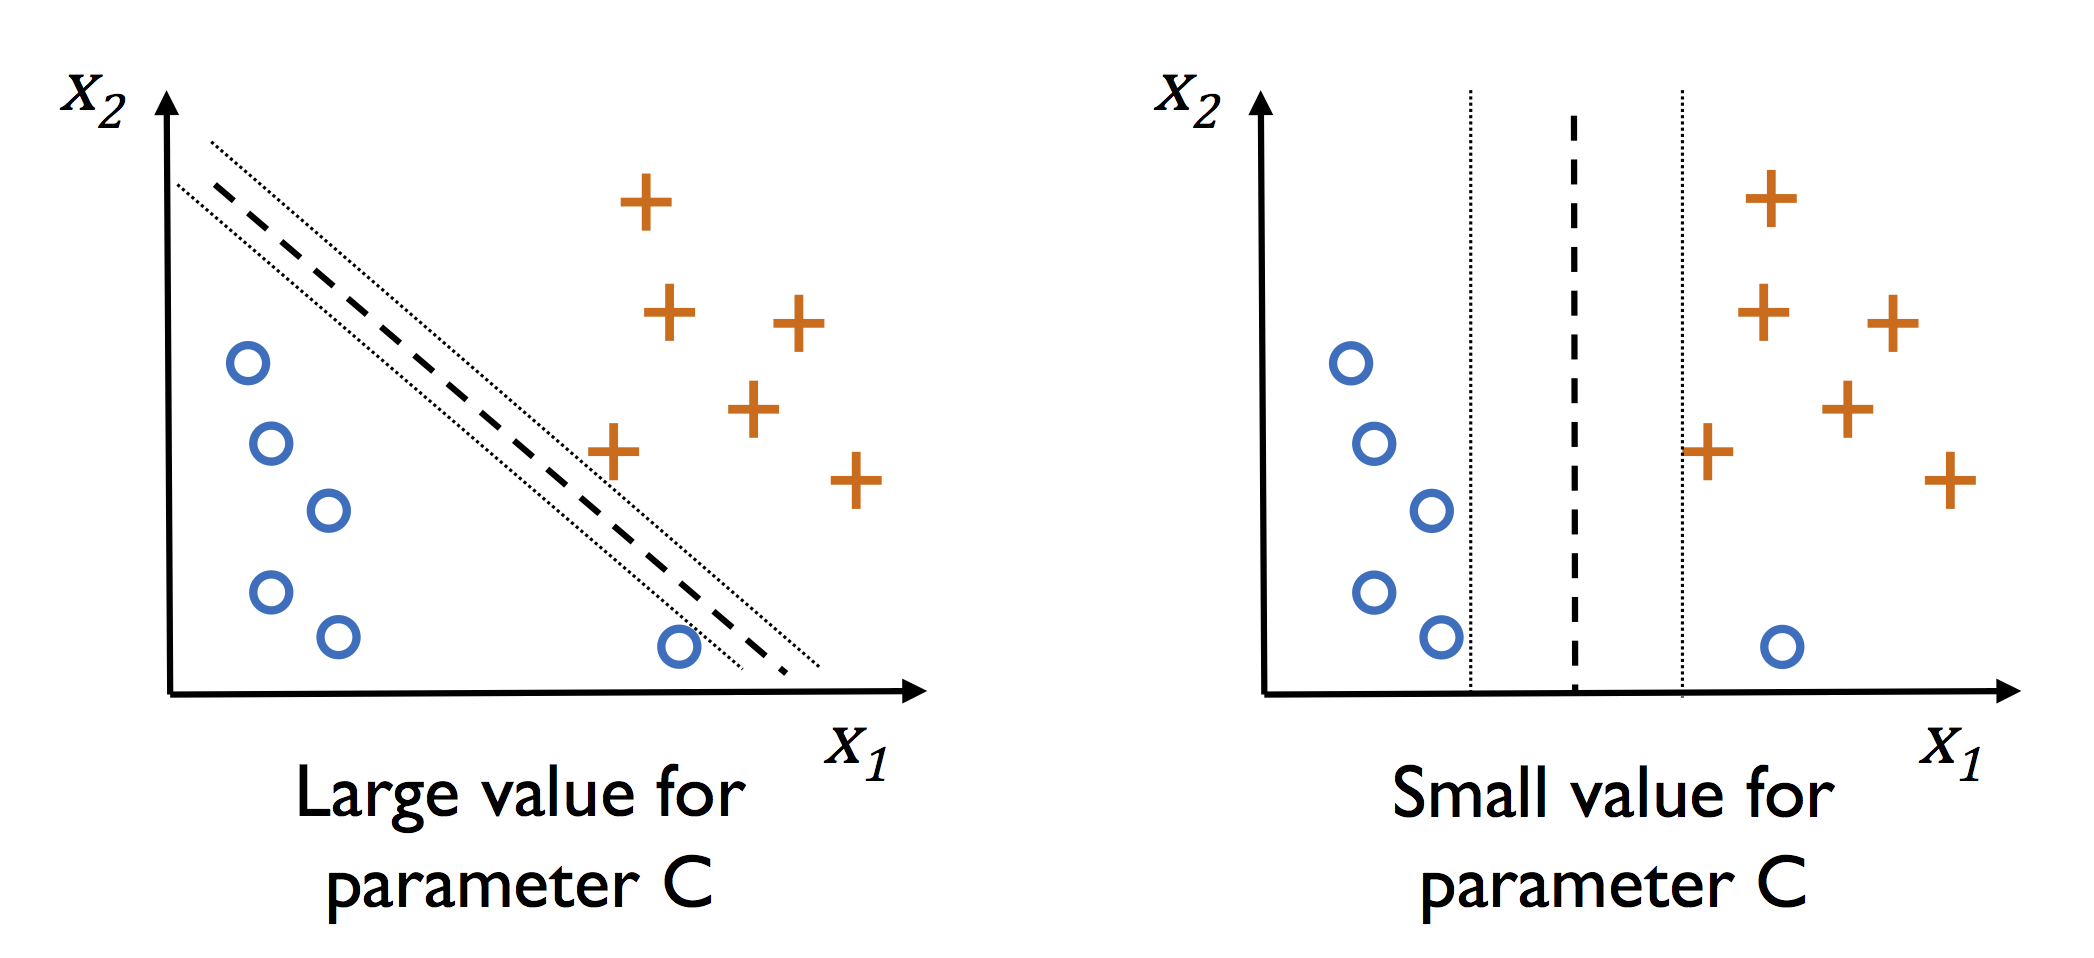
\includegraphics[width=80mm]{img/day02/fig06.png}
        \end{center}
    \end{figure}
\end{frame}

\begin{frame}{ロジスティック回帰との違い}
    実のところ、SVMはロジスティック回帰とよく似た結果を出す。
    しかし、以下の違いが存在するので使用の際は留意すること。
    \begin{alertblock}{ロジスティック回帰}
        モデルの構造が単純であるため扱いやすい。しかし、訓練データの尤度を最大化しようとするアルゴリズムため
        外れ値の影響を受けやすい。
    \end{alertblock}
    \begin{exampleblock}{SVM}
        マージンを最大化するアルゴリズムなため、外れ値に対して耐性を持つ。ロジスティック回帰と比べ
        モデルの構造が複雑なため扱いづらい。
    \end{exampleblock}
\end{frame}

\section{Kernel SVM}
\begin{frame}{カーネルSVM}
    SVMが機械学習モデルの中で高い人気を誇るもう1つの理由に、非線形分類の問題を解くための「カーネル化」が
    容易なことが挙げられる。ここではノイズ入りのXORデータセットを作成し、カーネルSVMで非線形分類を行う。
    \begin{figure}[b]
        \begin{center}
        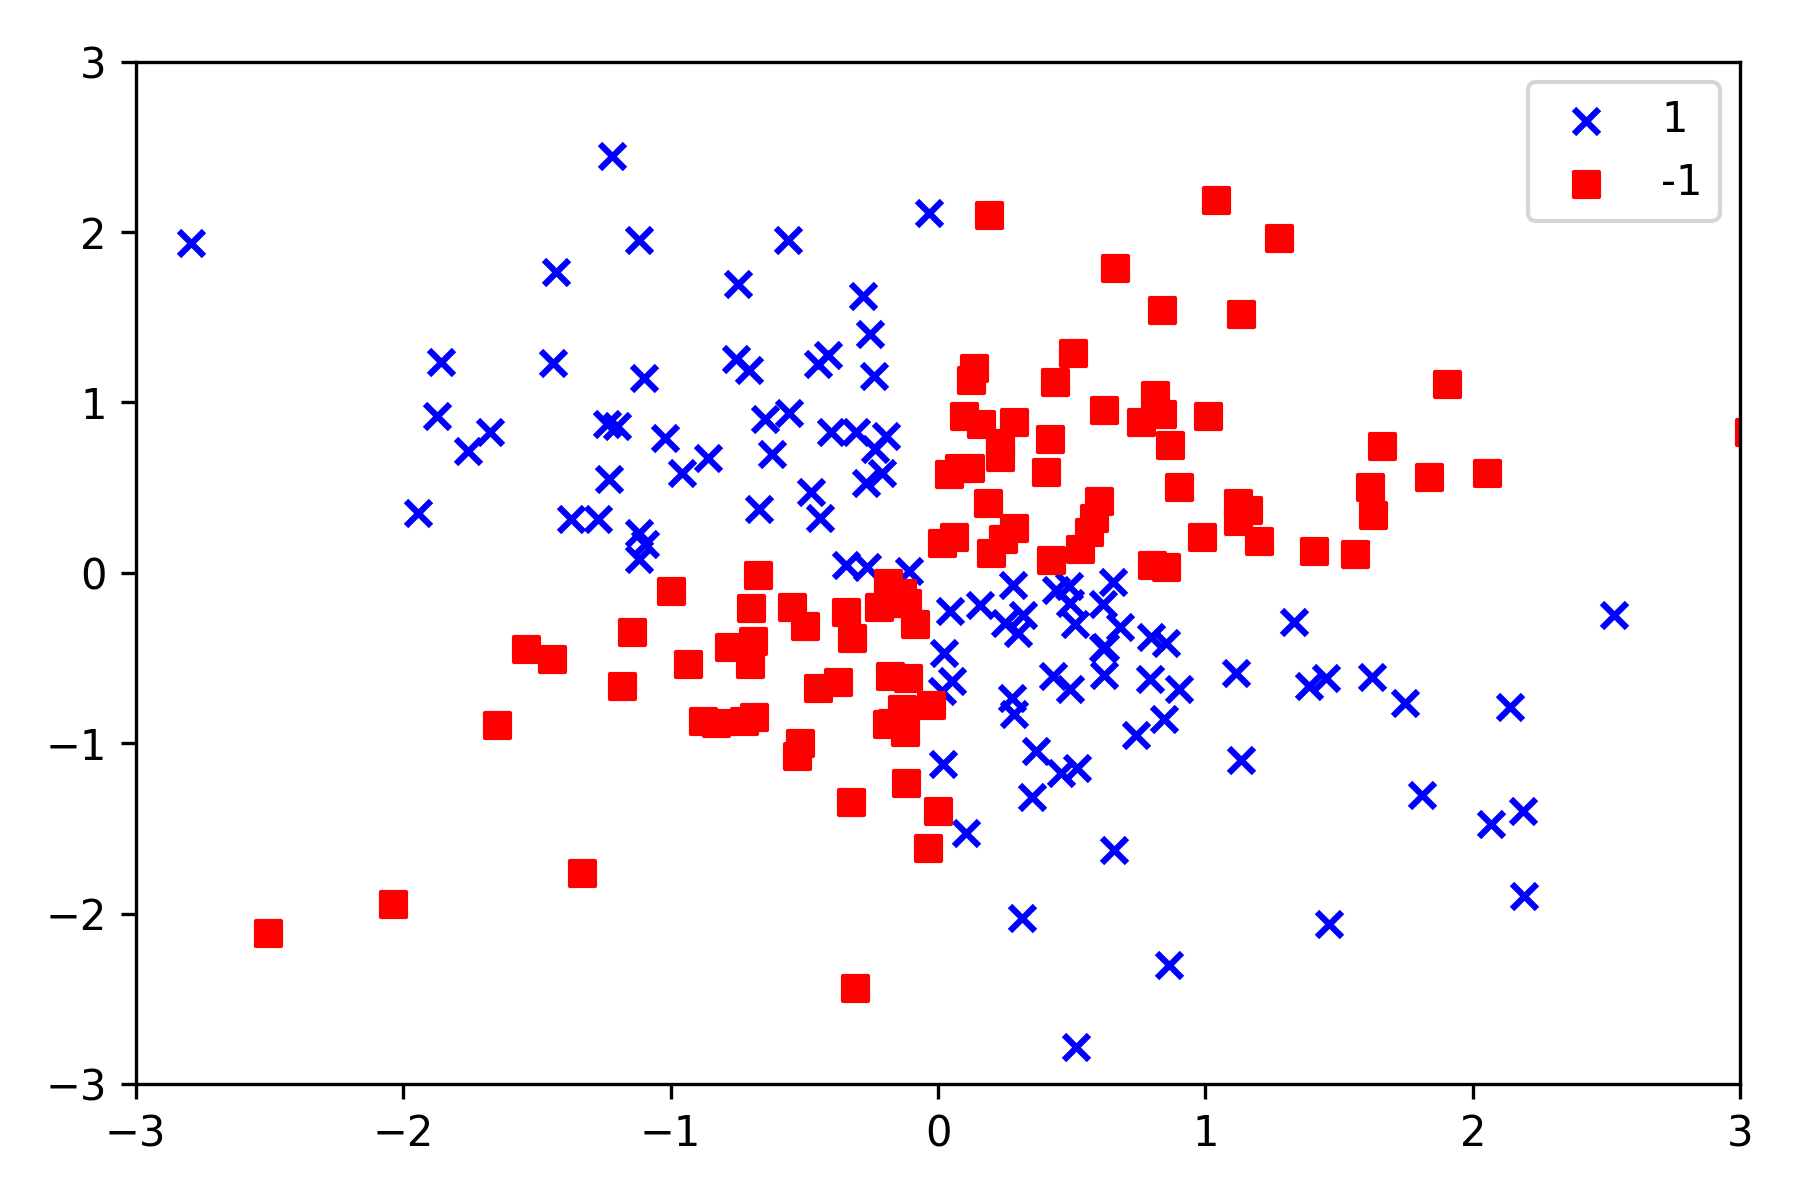
\includegraphics[width=70mm]{img/day02/fig07.png}
        \end{center}
    \end{figure}
\end{frame}

\begin{frame}{カーネルSVM}
    線形分離出来ないデータを処理するカーネル手法の主な考え方は、射影関数\(\phi\)を使ってそれらの組み合わせを
    高次元空間に写像し、線形分離できるようにすることである。\\
    この場合次の射影関数を使ってクラスを分離している。
    \begin{equation*}
        \phi(x_1, x_2) = (z_1, z_2, z_3) = (x_1, x_2, x_{1}^{2}+x_{2}^{2})
    \end{equation*}
    それを元の特徴量次元へ射影すると非線形の決定境界になる。
    \begin{figure}[b]
        \begin{center}
        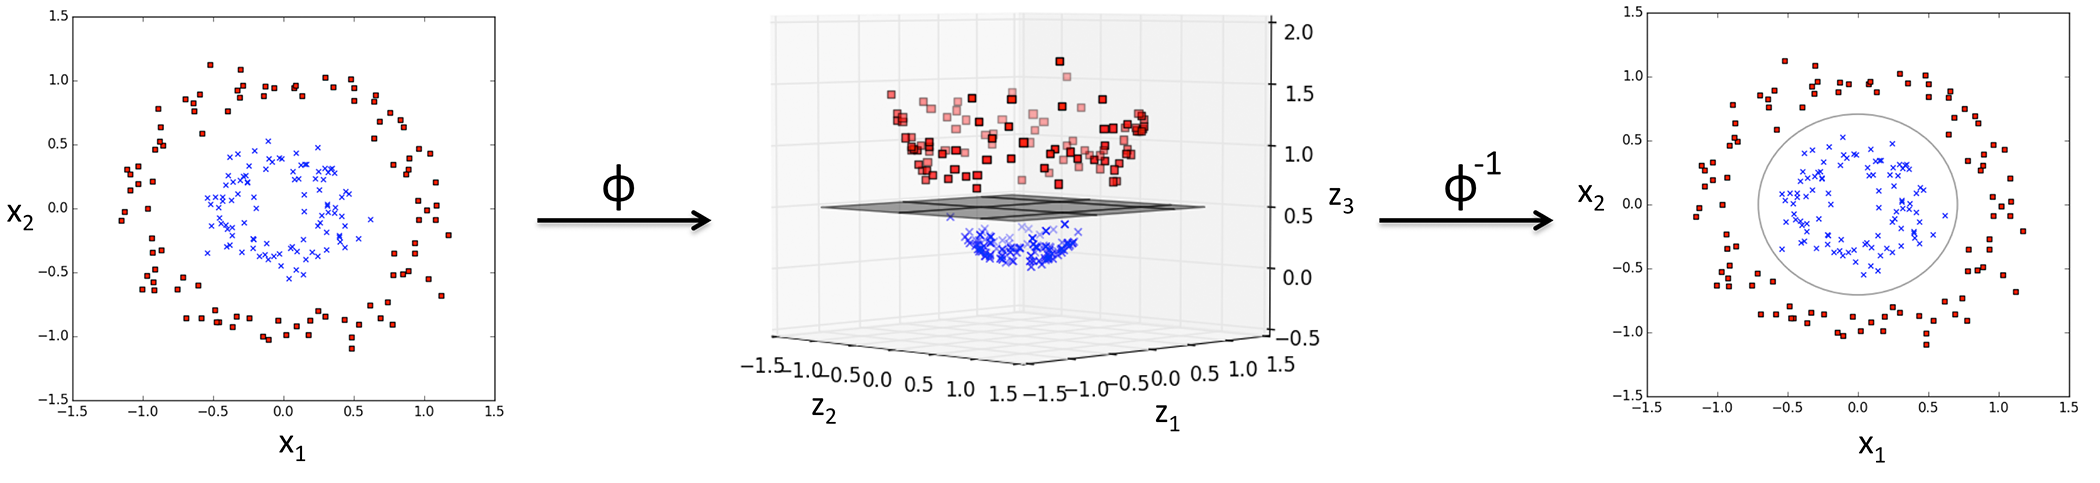
\includegraphics[width=150mm]{img/day02/fig08.png}
        \end{center}
    \end{figure}
\end{frame}

\begin{frame}{カーネルトリック}
    この写像手法は問題を抱えており、新しい特徴量を生成した場合計算量が大幅に増える。
    それは高次元の特徴量を扱う場合、無視できなくなる。\\
    カーネル手法ではベクトルのドッド積\(\bm{x}^{(i)T}\bm{x}^{(j)}\)を
    \(\phi(\bm{x}^{(j)})^T \phi(\bm{x}^{(j)})\)に置き換えているが
    このドット積を計算すると計算コストが発生するためカーネルを定義する。
    \begin{equation*}
        \mathcal{K} (\bm{x}^{(i)}, \bm{x}^{(j)}) = \phi(\bm{x}^{(j)})^T \phi(\bm{x}^{(j)})
    \end{equation*}
    最も広く使われているカーネルの1つが動径基底関数カーネルであり「RBFカーネル」、「ガウスカーネル」などと呼ばれ、
    このように表される。
    \begin{equation*}
        \mathcal{K} (\bm{x}^{(i)}, \bm{x}^{(j)}) 
        = \exp (-\gamma \Vert\bm{x}^{(i)} - \bm{x}^{(j)}\Vert^2), 
        \gamma = \frac{1}{2\sigma ^2}
    \end{equation*}
    ここで\(\gamma \)は最適化されるハイパーパラメータである。
\end{frame}

\section{多クラス分類}

\end{document}